\documentclass[12pt]{article}
\usepackage[left=1.0in,top=1.0in,right=1.0in,bottom=1.0in]{geometry} % Document margins
\usepackage{fancyhdr}
\pagestyle{fancy}
\fancyhead[LE,LO]{Braden Anderson (203744563) \& Alan Kha (904030522)}

\usepackage[all]{xy} % for arrow diagrams.

\usepackage{authblk}
\usepackage{listings}
\usepackage{color}

% tikz stuff (for fancy flowcharts)
\usepackage{tikz}
\usetikzlibrary{shapes,arrows}
% Define block styles
\tikzstyle{decision} = [diamond, draw, fill=blue!20,
	text width=4.5em, text badly centered, node distance=3cm, inner sep=0pt]
\tikzstyle{block} = [rectangle, draw, fill=blue!20,
	text width=5em, text centered, rounded corners, minimum height=4em]
\tikzstyle{line} = [draw, -latex']
\tikzstyle{cloud} = [draw, ellipse,fill=red!20, node distance=3cm,
	minimum height=2em]


\definecolor{green}{rgb}{0,0.5,0}
\definecolor{purple}{rgb}{0.58,0,0.82}
\definecolor{gray}{rgb}{0.5,0.5,0.5}

\lstdefinestyle{customc}{
	belowcaptionskip=1\baselineskip,
	breaklines=true,
	frame=L,
	xleftmargin=\parindent,
	language=C,
	showstringspaces=false,
	basicstyle=\footnotesize\ttfamily,
	keywordstyle=\bfseries\color{blue},
	commentstyle=\color{green},
	identifierstyle=\color{black},
	stringstyle=\color{purple},
	numbers=left,
	numbersep=7pt,
	rulecolor=\color{black},
}

\lstset{escapechar=@,style=customc}

\begin{document}
\lstset{language=C}

\title{Lab 1ab Design Project:\\ Attack and Defend Your Shell}
\author[1]{Braden Anderson}
\affil[1]{bradencanderson@gmail.com}
\author[2]{Alan Kha}
\affil[2]{akhahaha@gmail.com}

\maketitle

\begin{abstract}
Our Lab 1ab implementation is potentially exploitable. This document will show in what ways our implementation is exploitable, and the possible forms that some exploits might take. Lastly, we will discuss security improvements that will protect against malicious attackers.
\end{abstract}

\section{Introduction}
Lab 1 implements a shell interpreter for a small subset of POSIX grammar. An input script with valid syntax is read and executed similar to the command \texttt{sh script.sh}. There are some key differences between modern shells and our own -- most notably, we do not support flow control structures such as loops, if statements, and case switches. As we will discuss in later sections, an absence of loops simplifies design concerns (and, by extension, security concerns) considerably.

\section{Security Objectives}
The objective of this report is to investigate possible security flaws that a malicious user could use to attack the system running our shell. Vulnerabilities that could be used to harm the host system, in particular using a hostile input script, will be addressed. We will investigate and fix known bugs within our own program, ensuring robust behavior.


\section{Overall Design}
Our shell interpreter implemenation takes a pipeline approach:

\begin{displaymath}
\xymatrix{
Shell \: script \ar[r] & \framebox{Tokenization} \ar[r] & \framebox{Parsing} \ar[r] & Execution
}
\end{displaymath}

One exception to the strict pipelining approach is that our parser calls back to the tokenizer when it encounters subshells. For example, tokenizing the following expression:

\begin{displaymath}
\xymatrix{
\framebox{echo a \&\& ( echo b )} \ar[r] & \framebox{echo} \: \framebox{a} \: \framebox{\&\&} \: \framebox{echo	 b}
}
\end{displaymath}

In the previous example, \texttt{echo b} remains untokenized after the initial tokenization pass. It's stored internally as a "subshell" token, and during the parsing phase it's tokenized dynamically. The parser returns a forest of command trees to main(), and these command trees are executed serially by our execution model. Execution is managed through a recursive traversal of each tree.

So the expanded design for our shell interpreter (without the \texttt{-p} option) looks like: \\

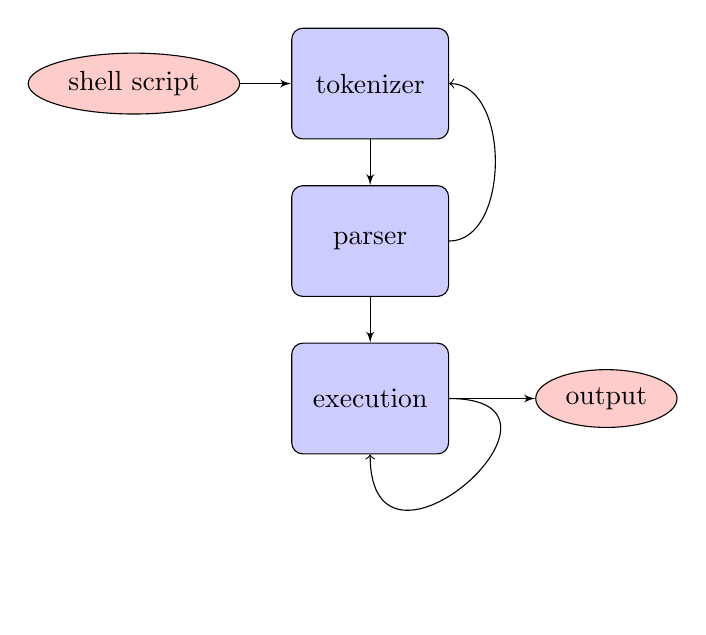
\begin{tikzpicture}[node distance = 2cm, auto]
	% Place nodes
	\node [block] (tokenizer) {tokenizer};
	\node [cloud, left of=tokenizer] (script) {shell script};
	\node [block, below of=tokenizer] (parser) {parser};
	\node [block, below of=parser] (execution) {execution};
	\node [cloud, right of=execution] (output) {output};
	% Draw edges
	\path [line] (script) -- (tokenizer);
	\path [line] (tokenizer) -- (parser);
	\path [line] (parser) -- (execution);
	\path [line] (execution) -- (output);
	\draw (parser) edge[out=0,in=0,->] (tokenizer);
	\draw[->] (execution) to [out = 0, in = 270, looseness = 4] (execution);
\end{tikzpicture}

\section{Threat Model}
This is where we model potential threats. This means that we use our security objectives to transform our overall application design into a system of components, data flows, and trust boundaries. Assumptions that we make:

\begin{enumerate}
	\item The shell interpreter is trusted, since we wrote all the code. However, it might enter an unsafe state.
	\item The user can be stupid or malicious.
	\item The operating system is trusted.
	\item The input can be intentionally or unintentionally malicious.
	\item Commands that have an interface outside our system -- for example, wget -- are potential sources of vulnerabilities.
\end{enumerate}

\section{Penetration Testing}
We performed several penetration tests centered around common vulnerabilities in C and shell scripts.

\subsection{Buffer Overflows}
 Certain C library functions, such as printf(), gets(), and memcpy() have well-known vulnerabilities\cite{formatstring,smashingthestack}. This is because the C language does not provide builtin, high-level support for buffers or cstrings. Shell interpreters are also common sources of system instability because they can modify portions of the file system.

Here is a program that is vulnerable to buffer overflows:
\begin{lstlisting}[frame=single]
int main(void) {
	char buf[10];
	int success = 0;

	printf("Enter string: \n");
	gets(buf);

	if (success)
		return 0;

	return 1;
}
\end{lstlisting}

Most buffer overflows are a result of trying to store data in a buffer of finite size.

During penetration testing we found a bug in our tokenizer where tokens can possibly include nullbytes. We found that a word with an internal nullbyte would be improperly tokenized. However, this behavior does not occur when tokenizing subshells, since we limit our subshell traversal using a call to strlen(), which truncates strings at the first nullbyte. The following table demonstrates this behavior: \\

\begin{tabular}{ | l | l | l | }
	\hline
		input & tokenized representation & output \\ \hline
		echo abc & `echo', `abc' & abc \\ \hline
		echo ab\textbackslash0c & `echo', `ab\textbackslash0c' & ab \\ \hline
		(echo ab\textbackslash0c) & `echo', `ab' & ab \\
	\hline
\end{tabular}\\

Fortunately we determined that this is not exploitable. This is because in the parsing stage we allocate space for the entire cstring, including nullbytes (as shown in the above table). So there is no possibility of a buffer overflow attack during the tokenization phase. Here is how we copy and allocate token space, with a dynamically sized buffer:

\begin{lstlisting}[frame=single]
size_t count = 0;
size_t word_size = 8;
char* word = checked_malloc(word_size);

do
{
	// load into word buffer
	word[count] = c;
	count++;

	// expand word buffer if necessary
	if (count == word_size)
	{
		word_size = word_size * 2;
		word = checked_grow_alloc(word, &word_size);
	}
	script++; index++; c = *script;
} while (is_word(c) && index < script_size);
\end{lstlisting}

All of our code after the tokenization phase deals with nullbyte-terminated strings, so space after the nullbyte is ignored in all strings. Furthermore, there is no vulnerability with the \texttt{-p} option because printf() deals with nullbyte-terminated strings.

\subsection{Format String Vulnerabilities}

We performed another penetration test by looking for format string vulnerabilities. Here are all usages of printf() in our implementation:

\begin{lstlisting}[frame=single]
	printf ("# %d\n", command_number++);
	printf (" \\\n%*s%s\n", indent, "", command_label[c->type]);
	printf ("%*s%s", indent, "", *w);
	printf (" %s", *w);
	printf ("%*s(\n", indent, "");
	printf ("\n%*s)", indent, "");
	printf ("<%s", c->input);
	printf (">%s", c->output);
\end{lstlisting}

All of the usages of printf() listed here make use of hard-coded format strings, therefore making us unsuccessful in finding a format string vulnerability.

\subsection{Inherently Bad Commands}
Commands that would harm the system and can be executed through the standard shell can likely be executed through our shell, and are vulnerabilities outside the scope of our security objectives.

A relatively benign yet poignant example of inherently bad commands the ease of deleting the shell interpreter itself, simply by inserting a single line \texttt{rm -rf timetrash} into the input script. The script is able to run to completion because the executable has already been loaded into memory. A slightly more ambitious attack could even delete the entire directory with \texttt{rm -rf ../time-travel-shell}. As undesirable as they, these commands are still legal commands that must be obeyed.

\subsection{Elevated permissions}
Processes in UNIX operating systems inherit the permissions of their parent process. This means that when executing the shell interpreter with superuser permission, great care must be taken to ensure that the input script is safe.

Normally, executing a script with the line \texttt{ls > /home/output} would return a failure as creating writing to the home directory requires superuser permission. However, when executing \texttt{sudo ./timetrash script}, the redirect commands successfully execute with root access.

\section{Robustness Analysis}
\begin{itemize}
	\item Input validation
	\item No fixed-size buffers
	\item No calls to printf() with uncontrolled format string
	\item No unsafe library functions
\end{itemize}

\section{Conclusion}
We have determined that it is unlikely for an attacker to be able to exploit our processing of the input script to create unwanted behavior, at least using buffer overflow or printf vulnerabilities.

The most likely avenue of attack would likely be through inherently bad commands, but preventing these is out of the scope of our program as they are problems inherent in any shell. Administrators who choose to use our interpreter for their system must take care to ensure only trusted users can execute scripts, and take special care when executing with superuser privileges.

% This is where code samples will go.
\appendix
\section{A shellcode exploit}
[fill in]

\begin{thebibliography}{9}

\bibitem{formatstring}
	scut/team teso,
	Exploiting Format String Vulnerabilities.
	Stanford University,
	Version 1.2,
	2001.

\bibitem{smashingthestack}
	Aleph One,
	Smashing the Stack for Fun and Profit.
	Phrack,
	Volume 7,
	1996.
\end{thebibliography}

\end{document}
